\documentclass[a4paper,14pt]{extarticle} \usepackage[utf8]{inputenc}
\usepackage[T1]{fontenc}
\usepackage[margin=2.5cm]{geometry}

% Fonte Caladea se existir, senão lmodern
\IfFileExists{caladea.sty}{
  \usepackage{caladea}
}{
  \usepackage{lmodern} }
\usepackage{ragged2e}
\usepackage{graphicx}
\usepackage[portuguese]{babel}
\usepackage{wrapfig}
\usepackage{hyperref}
\usepackage{fancyhdr}
\usepackage{xcolor}
\usepackage{rotating}
\usepackage{titlesec}
\usepackage{epigraph}
\usepackage{dirtytalk}
\usepackage{indentfirst} % Indenta o primeiro parágrafo após seções

% Ajuste do recuo de parágrafo
\setlength{\parindent}{1.5em}

% Centralizar títulos
\titleformat{\section}
  {\normalfont\centering\bfseries\Large}{\thesection}{1em}{}

\titleformat{\subsection}
  {\normalfont\centering\bfseries\large}{\thesubsection}{1em}{}

\titleformat{\subsubsection}
  {\normalfont\centering\bfseries}{\thesubsubsection}{1em}{}

% -------------- Símbolos de Versículo e Resposta --------------
% Definição do símbolo (a “barrinha” inclinada)
\makeatletter
\newcommand{\vers@resp@sym}{%
  \raisebox{0.2ex}{\rotatebox[origin=c]{-20}{$\m@th\rceil$}}%
}
% macro interna que sobrepõe a barrinha e a letra V ou R
\newcommand{\vers@resp}[2]{%
  {\ooalign{%
     \hidewidth\kern#1\vers@resp@sym\hidewidth\cr
     #2\cr
  }}%
}
% comandos públicos \versicle e \response
\DeclareRobustCommand{\versicle}{\vers@resp{-0.1em}{V}}
\DeclareRobustCommand{\response}{\vers@resp{0pt}{R}}
\makeatother
% ^------------- Símbolos de Versículo e Resposta -------------^

% Rodapé com imagem e página
\pagestyle{fancy}
% ---- Cabeçalho ------------
\fancyhf[C]{}
% ----- Rodapé --------------
\fancyfoot[LO,LE]{%
  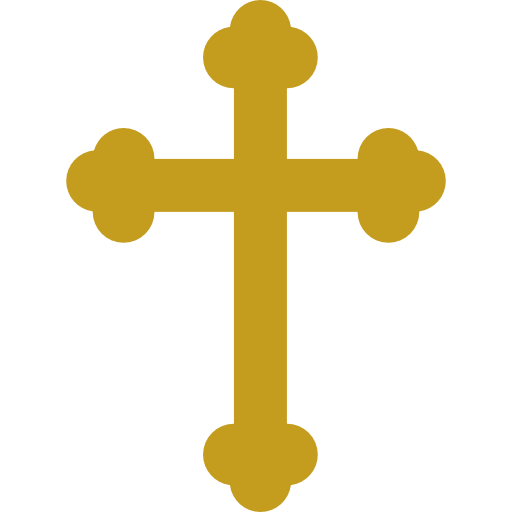
\includegraphics[scale=0.2]{assets/cross.png}\quad
  \textit{Novena a \textbf{Nossa Senhora do Bom Remédio}}
}
\fancyfoot[RO,RE]{\thepage}

\begin{document}


\subsection*{Novena a Nossa Senhora do Bom Remédio}

\say{
Em determinado momento, percebi que precisávamos de um edifício para reunir adoradores do Santíssimo Sacramento, pois o sustento de minha obra dependia dessa devoção. Então, comecei a novena de Nossa Senhora do Bom Remédio; no nono dia, apareceram alguns doadores e me ofereceram tudo o que eu precisava.
}

\par\noindent\rule{\textwidth}{0.4pt}

\tableofcontents
\thispagestyle{empty}

% --- Vida / Origem da Novena ---
\newpage

\section{Origem da Devoção}

Sob a bela invocação de Mãe do Bom Remédio,a Virgem Santíssima se nos apresenta como dispensadora dos auxílios sobrenaturais e materiais de que nós, insuficientes e miseráveis que somos, necessitamos em meio às penúrias deste vale de lágrimas.

\subsection{Mas por que “bom remédio”?}

A bem dizer, o termo remédio – que deriva do substantivo latino remedium, bem como do verbo remediare – denota uma solução ou lenitivo para qualquer espécie de necessidade. Com efeito, embora muito empregado para designar uma substância utilizada para sanar enfermidade físicas, refere-se também a tudo quanto pode prevenir, aliviar ou eliminar algum mal, mesmo moral ou espiritual.

É razoável, ademais, que os remédios sejam dispensados a um enfermo em proporção às moléstias que o acometem, pois ninguém busca curar-se de uma grave doença com o uso de simples analgésicos, e muito menos utiliza medicamentos fortes e de uso restrito no tratamento de leves incômodos.

Isto posto, perguntamo-nos: que “bom remédio” é este que Nossa Senhora nos oferece? E que tipo de mal ele visa combater?

\subsection{Jesus Cristo, a Cura do verdadeiro mal}

Devido à transgressão de nossos primeiros pais, o gênero humano foi acometido pela pior das enfermidades: o pecado. Como canta um belo hino gregoriano dedicado à Mãe de Deus, o universo estava “inteiro na amargura, inteiro na dor, inteiro no perigo”, pois “o inimigo tudo dominava completamente”; entretanto, pela Encarnação de Nosso Senhor Jesus Cristo, “foi dado ao mundo moribundo um remédio não humano, mas divino”. Afirma também o Pe. Jourdain que a Virgem Maria trouxe à terra Aquele que pode curar por completo o pior dos males: “Ela engendrou o Autor da salvação. O remédio onipotente, o único capaz de devolver à humanidade a saúde e a vida, saiu de Maria”.

Pois bem, se Maria nos deu esse remédio supremo, por que não esperaríamos d’Ela todos os demais “remédios” de que necessitamos? Como Mãe extremosa, Ela não poderia nos conceder grandes dádivas sobrenaturais sem estar atenta também às nossas pequenas carências de índole material. Estas mesmas carências, aliás, relacionam-se de forma íntima à origem e ao desenrolar da devoção a Nossa Senhora do Bom Remédio.

\subsection{Solução para um cruel impasse}

A Europa do século XII assistiu a interminável e encarniçada peleja entre os católicos e maometanos que, iniciada na Península Ibérica no século VIII prolongou-se por tempo indefinido. Durante séculos de embates, vários cristãos da Espanha, do sul da França e da Sicília foram feitos prisioneiros e desterrados para o norte da África e o Oriente Médio.

Estes filhos da Igreja, fadados à mais terrível escravidão, estavam alheios a qualquer esperança de resgate. Entretanto, a Providência Divina não tardaria em lhes enviar, por meio de uma alma eleita, a solução para o cruel impasse.

\subsection{Uma Ordem Religiosa em auxílio dos cativos}

De ascendência franco-espanhola, João da Mata veio à luz provavelmente no ano de 1160. Embora seus dados biográficos tenham-se perdido na noite dos tempos e sejam, portanto, incertos, acredita-se que ainda jovem ele presenciou os maus-tratos infligidos pelos muçulmanos aos cristãos no porto da cidade francesa de Marselha e, desde então, um forte desejo de trabalhar em favor destes infelizes firmou-se em seu espírito, levando-o a consagrar-se a Deus. Após estudar Teologia em Paris, foi ordenado sacerdote por volta dos trinta e três anos.

Narra uma antiga tradição que, durante a elevação da Hóstia Sagrada em sua primeira Missa, o Santo teve uma impressionante visão: o Salvador apareceu-lhe, trajado com uma túnica alva sobre a qual se desenhava uma bela cruz azul e vermelha, sustentando com as mãos dois prisioneiros cristãos. Ele manifestou o desejo de que fossem resgatados e, para isso, pediu ao sacerdote recém-ordenado que fundasse uma Ordem Religiosa em favor da redenção dos cativos. Depois dessa graça, João da Mata resolveu empregar sua vida na execução do pedido divino. Com o auxílio de um monge francês, São Félix de Valois, fundou a Ordem da Santíssima Trindade, aprovada pelo Papa Inocêncio III a 17 de dezembro de 1198.

Contudo, já nos primórdios de seu labor missionário ele teve de enfrentar um grande desafio de ordem material: onde encontrar os meios financeiros para o resgate dos cativos? Os infiéis apenas aceitavam libertar os detidos em troca de vultosas somas e, como reza o provérbio, “dinheiro não nasce em árvore”…

\subsection{Na aflição, o recurso necessário}

Conta-se que no ano de 1202, em Valência, o santo fundador encontrava-se profundamente angustiado pela escassez de recursos e implorava aos Céus uma intervenção. Foi então que a própria Maria Santíssima lhe apareceu e entregou um saco cheio de moedas, com as quais ele pôde resgatar muitos prisioneiros. O fato repetiu-se oito anos mais tarde, na cidade de Túnis.

Ora, o fundador não foi o único a receber a visita da Virgem. Na madrugada de 8 de setembro de 1212, festa da Natividade de Nossa Senhora, enquanto os raios da aurora penetravam lentos e majestosos pelos vitrais da capela do convento e os religiosos cantavam o Ofício Divino, Maria Santíssima apareceu a São Félix de Valois revestida com o hábito trinitário e rodeada de coortes angélicas. Entregou-lhe o escapulário da Ordem, manifestando o desejo de que este fosse imposto sobre os cativos resgatados.

Devido a estas aparições, Nossa Senhora do Bom Remédio é retratada com dois emblemas principais: o saquinho de moedas e o escapulário com uma cruz, cujas cores simbolizam a Santíssima Trindade: o branco, base e princípio de todas as cores, representa o Pai, que é ingênito; o azul, cor da carne humana machucada, faz alusão ao Filho, ferido em sua humanidade durante a Paixão; e o vermelho, figura do fogo divino que tudo consome, refere-se o Espírito Santo.

Em 1688 a Ordem da Santíssima Trindade proclamou Nossa Senhora, Mãe do Bom Remédio, como sua padroeira oficial. Quase três séculos depois, ela receberia caráter oficial na Igreja pela carta apostólica Sacrarium Trinitatis, do Papa João XXIII.

Fora dos muros do convento de Marselha, onde primeiro se venerou a Virgem sob esse título, logo as representações se multiplicaram. Uma das mais difundidas é a que se encontra hoje na Basílica de São Crisógono, em Roma, santuário confiado aos cuidados dos trinitários pelo Papa Pio IX em 1847. O autor do afresco, Giovanni Battista Conti, concluiu a pintura de estilo neobizantino no ano de 1944, em agradecimento à Santíssima Virgem Maria pela preservação de Roma dos flagelos da Segunda Guerra Mundial.

No Brasil, uma cópia deste piedoso retrato pode ser venerada na Basílica de Nossa Senhora do Rosário, em Caieiras, São Paulo. Posta em local de destaque, à direita do presbitério, a imagem evoca as origens da grande devoção dos Arautos do Evangelho a esta invocação mariana.
Como outrora Ela favoreceu o fundador dos trinitários…

Tendo recebido do Papa João Paulo II a aprovação pontifícia em fevereiro de 2001, os Arautos do Evangelho almejavam ardorosamente que a difusão de seu apostolado fosse a mais abrangente e frutífera possível. Para isso, Mons. João Scognamiglio Clá Dias, fundador da associação, desejava a construção de templos segundo o carisma que Deus lhe inspirara. Ele julgava esse passo indispensável para a consolidação da obra, a formação de seus membros e o desenvolvimento das atividades junto aos fiéis, pois as edificações materiais são capazes de transmitir doutrinas abstratas em figuras acessíveis e atraentes.

Durante uma viagem de apostolado ao Canadá no ano de 2003, alguns membros dos Arautos, entre eles o próprio fundador, foram convidados pela emissora EWTN para uma visita à sua sede, localizada em Birmingham, Alabama, nos Estados Unidos. Nesta ocasião, Mons. João pôde conhecer a principal promotora deste apostolado mundial, a célebre Madre Angélica, bem como o grande e suntuoso santuário por ela erigido. Desde então, estabeleceu-se entre ambos uma profunda amizade.

Ainda nesse encontro, o fundador dos Arautos do Evangelho, impressionado com a imponente construção e tendo em mente seus planos acima mencionados, perguntou à religiosa:

— Como a senhora obteve os recursos para construir esta maravilha?

E ela respondeu:

— Em determinado momento, percebi que precisávamos de um edifício para reunir adoradores do Santíssimo Sacramento, pois o sustento de minha obra dependia dessa devoção. Então, comecei a novena de Nossa Senhora do Bom Remédio; no nono dia, apareceram alguns doadores e me ofereceram tudo o que eu precisava.

Em seguida, ela lhe entregou a famosa novena.

Mais tarde, Mons. João confidenciou quais foram seus pensamentos naquela ocasião: “Vou precisar rezar trinta novenas, a fim de obter os meios para tudo o que necessitamos construir…” De fato, ele logo começou a recitá-la, e terminou rezando não apenas trinta, mas uma série ininterrupta de novenas!

Os milagres não se fizeram esperar. As primeiras construções dos Arautos do Evangelho, entre elas a Basílica de Nossa Senhora do Rosário, são hoje uma prova incontestável da assistência miraculosa da Mãe do Bom Remédio que, como outrora a São João da Mata e a São Félix de Valois, veio em auxílio de Mons. João e de sua obra.

Transido de gratidão a Maria Santíssima ao contemplar o início das edificações que tanto desejava, Mons. João comentou: “Como tudo isso foi possível? Se me perguntarem, só tenho uma coisa a dizer: pela fidelidade à novena perpétua de Nossa Senhora do Bom Remédio, que nós vamos manter até o fim do mundo”. Desde então, a novena passou a ser promovida em todas as casas dos Arautos.

\subsection{Invoquemo-La com confiança filial!}

Crises espirituais, problemas familiares, enfermidades, dificuldades financeiras… Quem está isento dos males desta vida?

Como a mais atenciosa das mães e verdadeira Médica Celeste, Maria Santíssima nos acompanha sempre com seu olhar terno e compassivo, e está pronta a nos socorrer a todo instante. Se nunca se ouviu dizer que alguém tenha recorrido a Ela e fosse desamparado, não seremos nós os primeiros!

Eis a lição que nos dá Nossa Senhora do Bom Remédio. Quando, pois, a Providência Divina nos visitar com sofrimentos, lembremo-nos de que basta invocá-La com confiança filial e obteremos tudo quanto necessitarmos. E, se Ela não puder nos livrar da dor, estará ao nosso lado consolando-nos e dispensando-nos graças abundantes para carregarmos nossa cruz com fidelidade.

\newpage

% --- Orações Diárias ---
\newpage

\section{Novena a Nossa Senhora do Bom Remédio}
\subsection*{Oração para Todos os Dias}

Ó Rainha do Céu e da Terra, Santíssima Virgem, nós Vos veneramos. Vós sois a Filha bem-amada do Deus Altíssimo, a eleita Mãe do Verbo Encarnado, a Imaculada Esposa do Espírito Santo, o sagrado Vaso da Altíssima Trindade.

Ó Mãe do Divino Redentor, que, sob o título de Nossa Senhora do Bom Remédio, vindes em ajuda de todos os que Vos invocam, estendei a nós a vossa proteção maternal. Dependemos de Vós, ó querida Mãe, como filhos sem ajuda e necessitados dependem de mãe terna e cuidadosa.

  \textbf{Ave Maria…}

Nossa Senhora do Bom Remédio, fonte de ajuda infalível, permiti-nos retirar de vosso tesouro de graças, nos momentos de necessidade, tudo quanto precisarmos. Tocai os corações dos pecadores, para procurarem a reconciliação e o perdão. Confortai os aflitos e os abandonados, ajudai aos pobres e aos que perderam a esperança, amparai os enfermos e os que sofrem. Possam eles ser curados de corpo e alma, e fortalecidos no espírito para suportar seus sofrimentos com paciente resignação e fortaleza cristã.

  \textbf{Ave Maria…}

Querida Senhora do Bom Remédio, fonte de ajuda infalível, vosso Coração compassivo conhece o remédio para toda aflição e miséria que encontramos na vida. Ajudai-nos, com vossas orações e intercessão, a encontrar remédio para nossos problemas e necessidades, especialmente (faça aqui o pedido que deseja.)

De nossa parte, ó amorosa Mãe, nós nos comprometemos a um estilo de vida mais intensamente cristão, a uma observância mais cuidadosa da Lei de Deus, a sermos mais conscientes em cumprir as obrigações do nosso estado de vida, e a esforçar-nos para sermos instrumentos de salvação neste mundo arruinado.

Querida Senhora do Bom Remédio, nós Vos pedimos que estejais sempre presente junto a nós e, por vossa intercessão, possamos gozar de saúde de corpo, de paz de espírito, e crescer na Fé e no amor ao vosso Filho, Jesus.

\[
  \textbf{Pai-Nosso, Ave-Maria, Glória Ao Pai.}
\]

\response Rogai por nós, ó Santa Mãe do Bom Remédio.

\versicle Para que possamos aprofundar nossa dedicação ao vosso Filho e reavivar o mundo com o seu Espírito. 


\vfill

\begin{center}
\subsection*{Fontes:}
Adaptado de: \underline{\href{https://revista.arautos.org/mae-do-bom-remedio-remedio-para-todas-as-aflicoes/}{Revista dos Arautos do Evangelho}}
\end{center}


\end{document}
